\documentclass{report}
\usepackage[utf8]{inputenc}
\usepackage{amsmath}
\usepackage{relsize}

% **********************************************************
% Document Settings                                        *
% **********************************************************
\usepackage{geometry}
\geometry{a4paper, margin=0.6in}

\usepackage{graphicx}
\graphicspath{{../outputs/light/}}

\usepackage{minted}
% \usemintedstyle{emacs}

\usepackage{fancyhdr}
\pagestyle{fancy}
\fancyhf{}
\lhead{Numerical Methods}
\rhead{Suman Mondal}
% \lfoot{\href{https://github.com/thatsuman/ccpcst-assignment.git}{View on Github}}
\lfoot{\href{https://github.com/thatsuman}{github.com/thatsuman}}
\rfoot{Page \thepage}

\usepackage{hyperref}
\hypersetup{
colorlinks=true,
linkcolor=blue,
filecolor=magenta,
urlcolor=blue,
}
\urlstyle{same}

\usepackage{fontspec}
% \setromanfont{Source Sans Pro}
% \setmonofont{Cascadia Code PL}


% macros start here
% problem
\newcommand{\problem}[3]{
  \section{#3}
    \underline{{\LARGE Source Code :}}
    \inputminted[breaklines,fontsize=\Large]{c}{#1.c}
    \bigbreak
    \noindent
    \underline{{\LARGE Program Output :}}
    \bigbreak
    \noindent
    \includegraphics[width=110mm,scale=0.5]{#2}
% \newpage
}
% subproblem
\newcommand{\subproblem}[3]{
  \subsection{#3}
    \underline{\emph{\Large Source Code :}}
    \inputminted[breaklines]{c}{#1.c}
    \bigbreak
    \noindent
    \underline{\emph{\Large Program Output :}}
    \bigbreak
    \noindent
    \includegraphics[width=110mm,scale=0.5]{#2}
% \newpage
}
% macros end here

% **********************************************************
% document begin here

\begin{document}
\begin{titlepage}
  \begin{center}
    \vspace*{2cm}
    
\includegraphics[width=0.3\textwidth]{logo}\\
    \vspace{0.5cm}
    {\huge \textbf{CENTRAL CALCUTTA POLYTECHNIC}}\\
    \vspace{0.4cm}
    21, Convent Road, Philips, Sealdah, Kolkata, West Bengal 700014\\
    \vspace{0.8cm}
    {\Large \textsc{dept. : computer science and technology}}
  \end{center}
  \vspace{1.2cm}
  \textsc{
    \huge
    \begin{itemize}
      \item name : suman mondal
      \item roll : dccpcsts5
      \item number : 10005537
      \item reg number : d192005242
      \item subject : java programming
      \item session : 2021 - 2022
      \item email : suman.mondal@outlook.in
    \end{itemize}
  }

\end{titlepage}

\pagenumbering{roman}
\newpage
\large{\tableofcontents}
% \tableofcontents
\clearpage
\pagenumbering{arabic}

\chapter{Numerical Methods Assignments}

\subsection{Write a C Program to find out the value of f(2.35) using Newton's Forward Interpolation Formula from the following table}
\begin{center}
\begin{tabular}{c|c|c|c|c|c}
  x: & 2.00 & 2.25 & 2.50 & 2.75 & 3.00 \\
  f(x): & 9.00 & 10.06 & 11.25 & 12.56 & 14.00 
\end{tabular}
\end{center}
\bigbreak
\underline{\emph{\Large Source Code :}}
\inputminted[breaklines]{c}{../codes/Q01.c}
\bigbreak
\noindent
\underline{\emph{\Large Program Output :}}
\bigbreak
\noindent
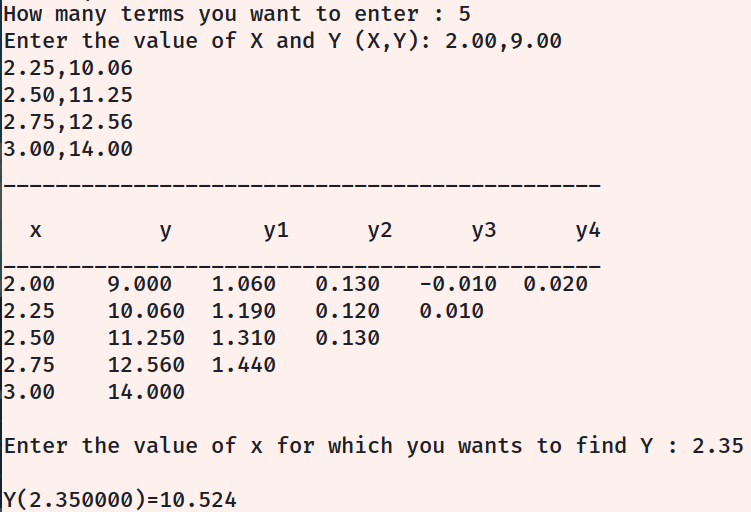
\includegraphics[width=110mm,scale=0.5]{../outputs/light/Q01.png}

\subsection{Write a C Program to find out the value of f(4.25) using Newton's Backward Interpolation Formula from the following table}
\begin{center}
\begin{tabular}{c|c|c|c|c|c}
  x: & 2.5 & 3.0 & 3.5 & 4.0 & 4.5 \\
  f(x): & 9.75 & 12.75 & 15.70 & 19.52 & 23.75 
\end{tabular}
\end{center}
\bigbreak
\underline{\emph{\Large Source Code :}}
\inputminted[breaklines]{c}{../codes/Q02.c}
\bigbreak
\noindent
\newpage
\underline{\emph{\Large Program Output :}}
\bigbreak
\noindent
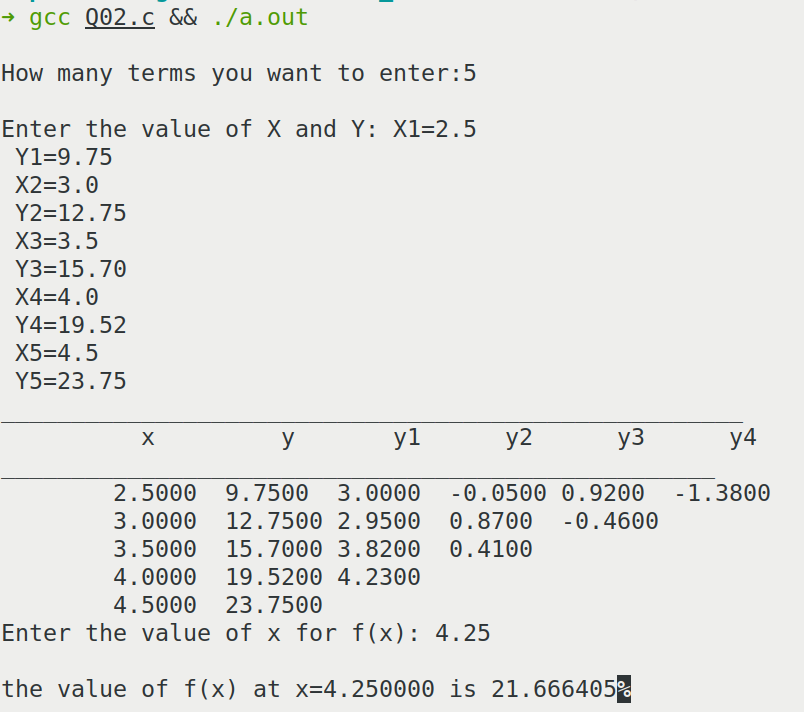
\includegraphics[width=110mm,scale=0.5]{../outputs/light/Q02.png}

\subsection{Write a C Program to find out the value of f(4.25) using Newton's Divide Difference Interpolation Formula from the following table}
\begin{center}
\begin{tabular}{c|c|c|c|c|c}
  x: & 2.5 & 3.0 & 4.5 & 4.75 & 6.0 \\
  f(x): & 8.85 & 11.45 & 20.66 & 22.85 & 38.60 
\end{tabular}
\end{center}
\bigbreak
\underline{\emph{\Large Source Code :}}
\inputminted[breaklines]{c}{../codes/Q03.c}
\bigbreak
\noindent
\newpage
\underline{\emph{\Large Program Output :}}
\bigbreak
\noindent
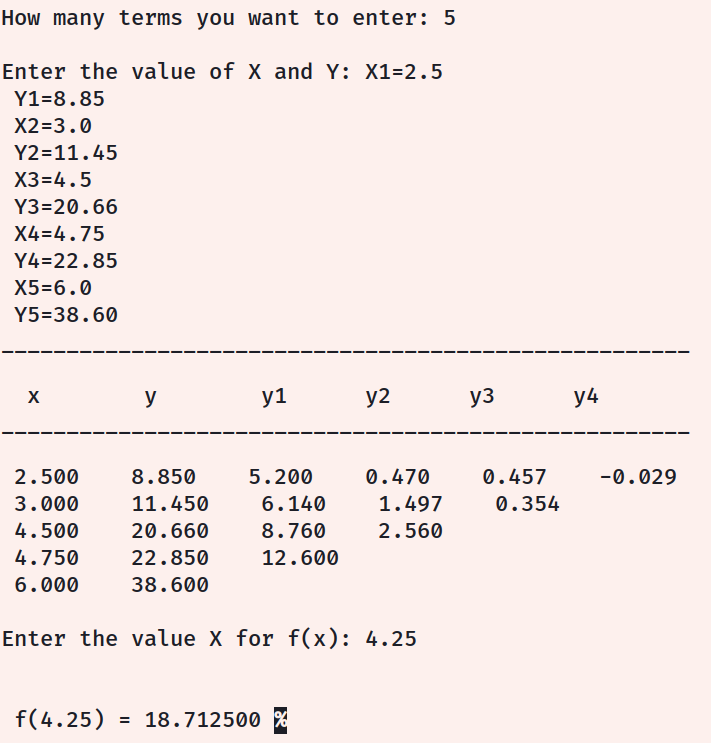
\includegraphics[width=110mm,scale=0.5]{../outputs/light/Q03.png}

\subproblem{../codes/Q04}{Q04}{Write a C Program to evaluate $\int_{2}^{1} \frac{1}{1+x^2} \,dx$ using Trapezoidal rule with 6 intervals}

\subproblem{../codes/Q05}{Q05}{Write a C Program to evaluate $\int_{2}^{1} \frac{x}{1+x} \,dx$ using Simpson's 1/3rd Rule with 6 intervals}

\subproblem{../codes/Q06}{Q06}{Write a C Program to find the root of the equation $x^3 + x^2 + x + 7 = 0$ using Bisection Method}

\subproblem{../codes/Q07}{Q07}{Write a C Program to find the root of the equation $x^3 - x -3 = 0$ using Newton Raphson Mehtod}


\end{document}
